\section{Methods}
\label{sec:formatting}
\subsection{Datasets}

In order to take into account movement characteristics to help identify smoke, analysts use multi-frame animations of the satellite imagery. The resulting annotations primarily have time windows over multiple hours, with an average of 3 hours of imagery represents one smoke plume annotation. Since the goal of these annotations is to show the general coverage over that time span, as shown in figure \ref{timelapse}, the smoke boundaries don't often match up with the satellite imagery over the entire time window. One way to approach this problem would be to use all the satellite images the analysts used as input. Since the timespans are non-uniform, this would vary the length in imagery inputs into the model, which would be difficult with a CNN architecture. Moreover, this would require a large amount of additional memory and computational resources. Instead of using the original analysts' many satellite image inputs to one annotated output, we develop a one-to-one input-to-output by finding the optimal singular satellite image input to represent the annotation. 

\begin{figure*}
    \centering
    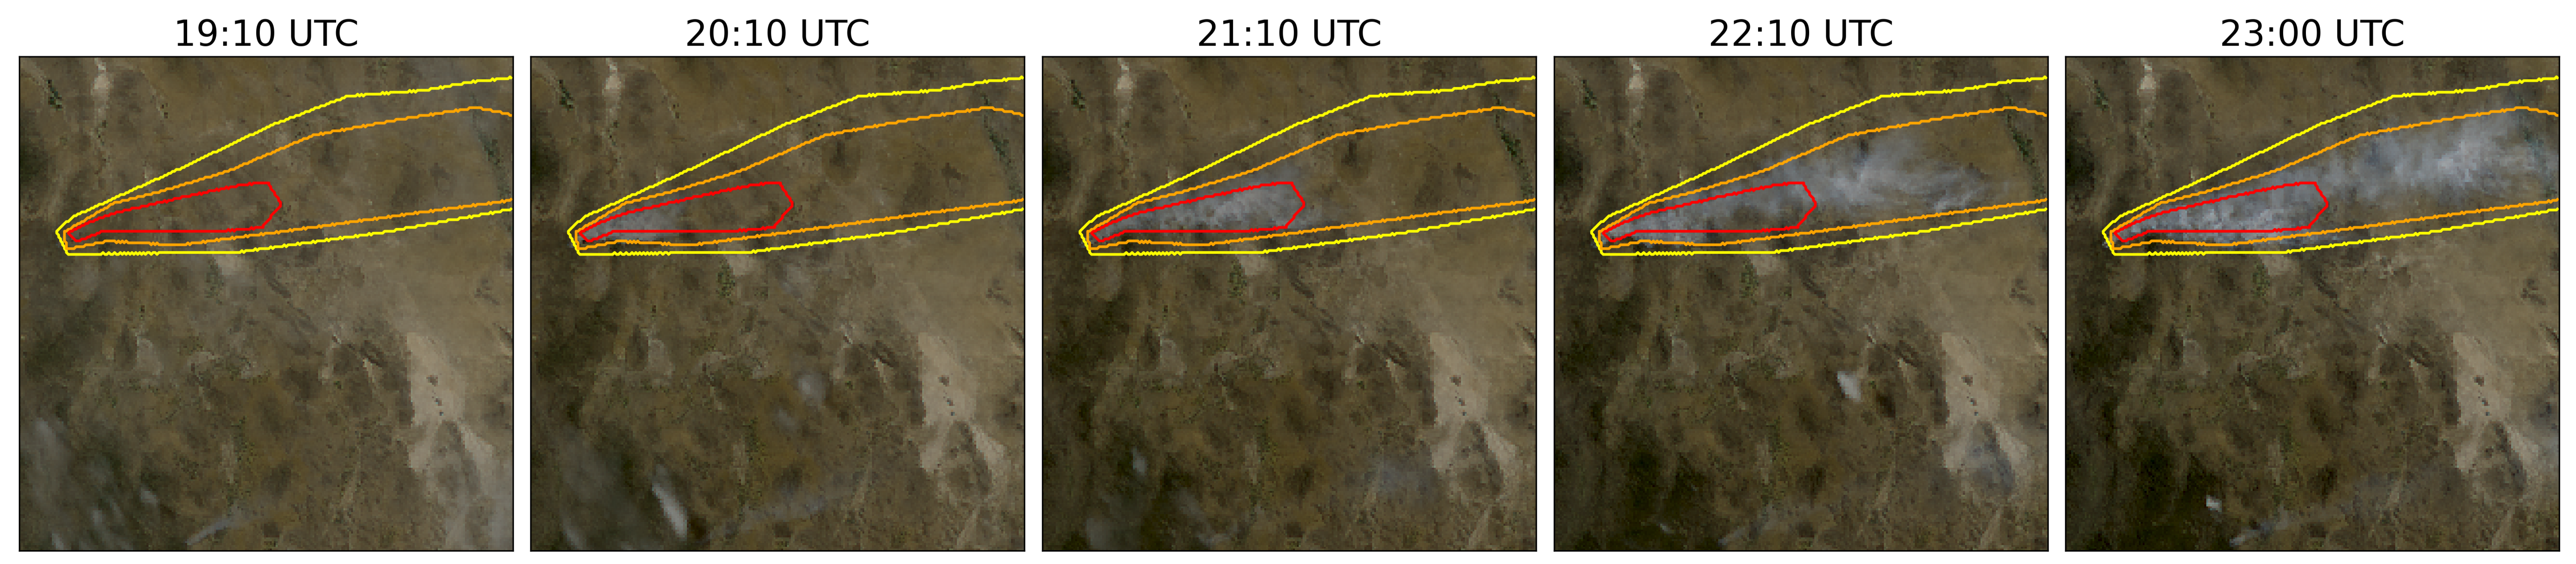
\includegraphics[width=\linewidth]{figures/TIMELAPSE_FINAL2.png}
    \caption{True color GOES-East imagery from May 5th, 2022, Southeast New Mexico (\(31.38^{\circ}\)N, \(107.87^{\circ}\)W) during the start of the Foster Fire. The red, orange and yellow lines represent the heavy, medium and low density HMS smoke annotations that span 19:10\textendash23:00 UTC.}
    \label{timelapse}
\end{figure*}



For the set of smoke annotations, \(\mathcal{Y}\), \(y \in \mathcal{Y}\) uses one or more \(x \in \mathcal{X}\) where \(\mathcal{X}\) is the entire set of satellite imagery corresponding to the set of time windows defined by the labels. In order to develop a one-to-one data-to-label dataset, we apply pseudo-labeling to develop a subset of \(\mathcal{X}\), denoted as \(\mathcal{X}_p\), that has a one-to-one ratio such that \(|\mathcal{X}_p| = |\mathcal{Y}|\), where we choose the satellite image that has the maximum overlap between the geolocation of smoke in the imagery and the analyst annotation.

But in order to create pseudo-labels we need an initial parent model, \(f_{\circ}\). To train \(f_{\circ}\), we need a way of choosing \(x \in \mathcal{X}\) that has a higher chance than random selection of being representative of \(y\). Discussed in further detail in the Mie-Derived Dataset subsection, we do this by making a series of physics-driven choices on which satellite and timestamp would give the optimal angle between the sun, smoke and satellite to produce the strongest smoke signature for the geolocation and timestamp of the smoke plume. This dataset, \(\mathcal{X}_M\) tells us that if there is smoke present during the entire time window, which timestamp would give the highest smoke signal-to-noise ratio. 

But more importantly than knowing the timestamp for maximum signal-to-noise, we want to know which image actually has smoke present within the smoke label boundaries. We used \(\mathcal{X}_M\) to train \(f_{\circ}\), to identify smoke in satellite imagery, and then use that \(f_{\circ}\) to create pseudo-labels of each satellite image in a given annotation's time-window. From those results, the optimal satellite image is chosen based on which image's pseudo-labels has the greatest overlap with the analyst annotation.




\subsubsection{Satellite Imagery} 

The GOES satellites are operated by NOAA in order to support meteorology research and forecasting for the United States. We use the latest operational satellites, GOES-16 (East), 17 and 18 (West) that each carry the ABI, that measure 16 bands between the visible and infrared wavelengths. In improvement to the GOES predecessors, imagery is collected every 5 minutes for the contiguous United States and every 10 minutes for the full disk. Using PyTroll, a Python framework for processing satellite data \cite{satpy}, we input bands 1-3 (Table \ref{rgb_bands}) to a GOES specific true color composite algorithm \cite{true_color} to develop a, 1km resolution, true color image representation, similar to what is seen by HMS analysts. As discussed in further detail in the next section, the highest signal-to-noise ratio will come from the smallest wavelengths of light, larger wavelengths have lower smoke signal and higher noise (figure \ref{bands}). For that reason, we only include the first 3 out of 16 available bands of data.

\begin{table}
    \caption{To create a true color image, we use the following bands from the ABI Level 1b CONUS (ABI-L1b-RadC) product.}\label{rgb_bands}
    \centering
        \begin{tabular}{ccccrrcrc}
            \toprule
            band & description & center \(\lambda\)($\mathrm{\mu m}$) & resolution (km)\\
            \midrule
            C01 &  blue visible & 0.47 & 1 \\
            C02 & red visible & 0.64 & 0.5 \\
            C03 & veggie NIR & 0.865 & 1 \\
            \bottomrule
        \end{tabular}
\end{table}


\subsubsection{Mie-Derived Dataset}

We used a physics-informed approach in selecting the initial GOES dataset, \(\mathcal{X}_M\), which we call the Mie-derived dataset, for training an initial parent model, \(f_{\circ}\), where if \(\mathcal{X}\) represents all the GOES imagery corresponding to the HMS smoke annotation time window, \(\mathcal{X}_M \subset \mathcal{X}\). Prior GOES ABI datasets for machine learning applications often include data from only one of the two GOES-series satellites, commonly opting for GOES-East \cite{smoke_goes}, \cite{wildfire_detect}, \cite{goes_conv}. Rather than using one satellite or the cumulative data from both GOES-West and GOES-East images, we select between one or the other based on the solar zenith angle. For smoke identification, this approach can achieve a much higher signal-to-noise than imaging the earth’s surface from an arbitrary angle. The elastic scattering of light is the primary mechanism to account for - while the atmosphere is composed of molecules with size \(<\)1nm, smoke particles can vary from 100 nm -- 10 \(\mu\)m in diameter, \(d\). The GOES ABI covers spectral bands from 0.47 \(\mu\)m -- 13.3 \(\mu\)m, so atmospheric and smoke particle sizes occupy two very different regimes with respect to the imaging wavelength \(\lambda\). In the extreme limit of \(\lambda \gg d\), the physics of scattering of light off a small sphere is captured by Rayleigh scattering. This process has two critical consequences: (1) the scattering cross section of light is strongly wavelength dependent (scaling with \(\lambda^{-4}\)), meaning that photons with wavelength closer to the ultraviolet are scattered more strongly than infrared photons. (2) the scattering cross section scales with an angular dependent cross section of \((1 + \cos^2 \theta)\). Scattered photons follow the emission distribution of a radiating dipole, scattering more strongly in the forward and backwards directions \((\theta = 0,\pi)\)than orthogonal to the direction of propagation \((\theta = \pi/2, 3\pi/2)\), see figure \ref{mei} for a Rayleigh scattering schematic.


\begin{figure}
    \centering
    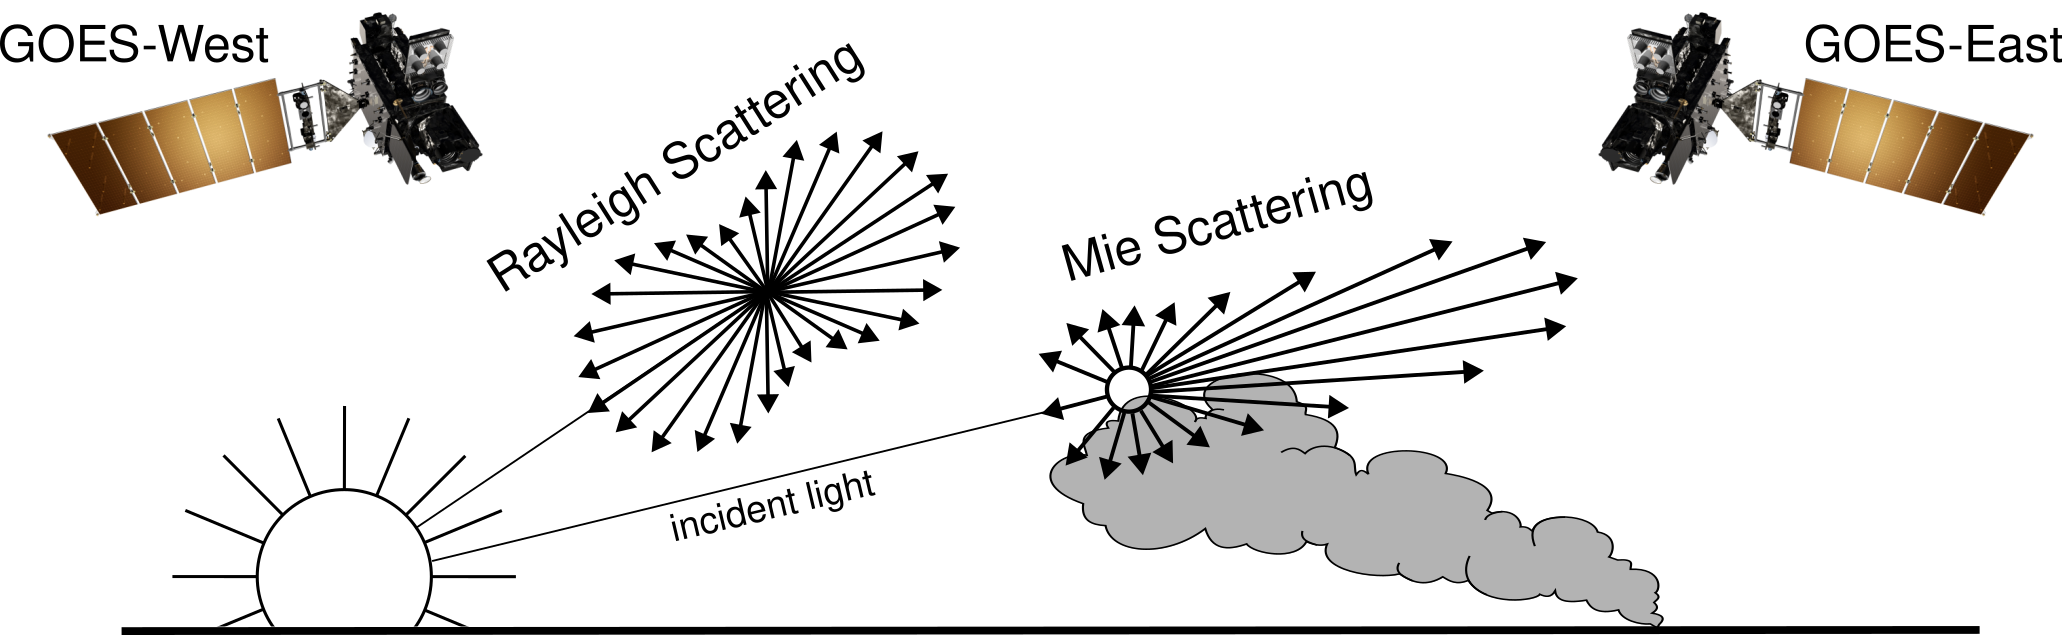
\includegraphics[width=8cm]{figures/mei.png}
    \caption{If the particle size is \(<\frac{1}{10}\) the wavelength of the interacting light, then the primary scattering will be Rayleigh. Mie scattering is the predominant scattering mechanism when the particle size is larger than the wavelength of light. This schematic demonstrates that when the sun is setting in the West, the Mie scattering will predominately forward scatter towards GOES-East.} \label{mei}
\end{figure}

The significance of these scalings is that the observer, or detector, will receive blue photons in most directions orthogonal to the source. Equivalently, photons traveling colinearly with line of sight to the emission source will mostly have wavelengths in the infrared band. In the converse regime of \(d > \lambda\), the elastic scattering of light against matter is modeled through Mie scattering. In comparison to Rayleigh scattering, Mie scattering is largely wavelength-independent and has a more complicated radiation pattern where the cross section has a maximal amplitude in the forward direction. An observer downstream of this scatterer will collect more photons than one positioned directly behind it. In the context of smoke identification, a sunrise or sunset will lead to a higher Mie scattered signal in GOES-West and GOES-East respectively, as shown with a smoke plume producing a stronger signal in GOES-East imagery near sunset in figure \ref{16_vs_17}.

\begin{figure}
    \centering
    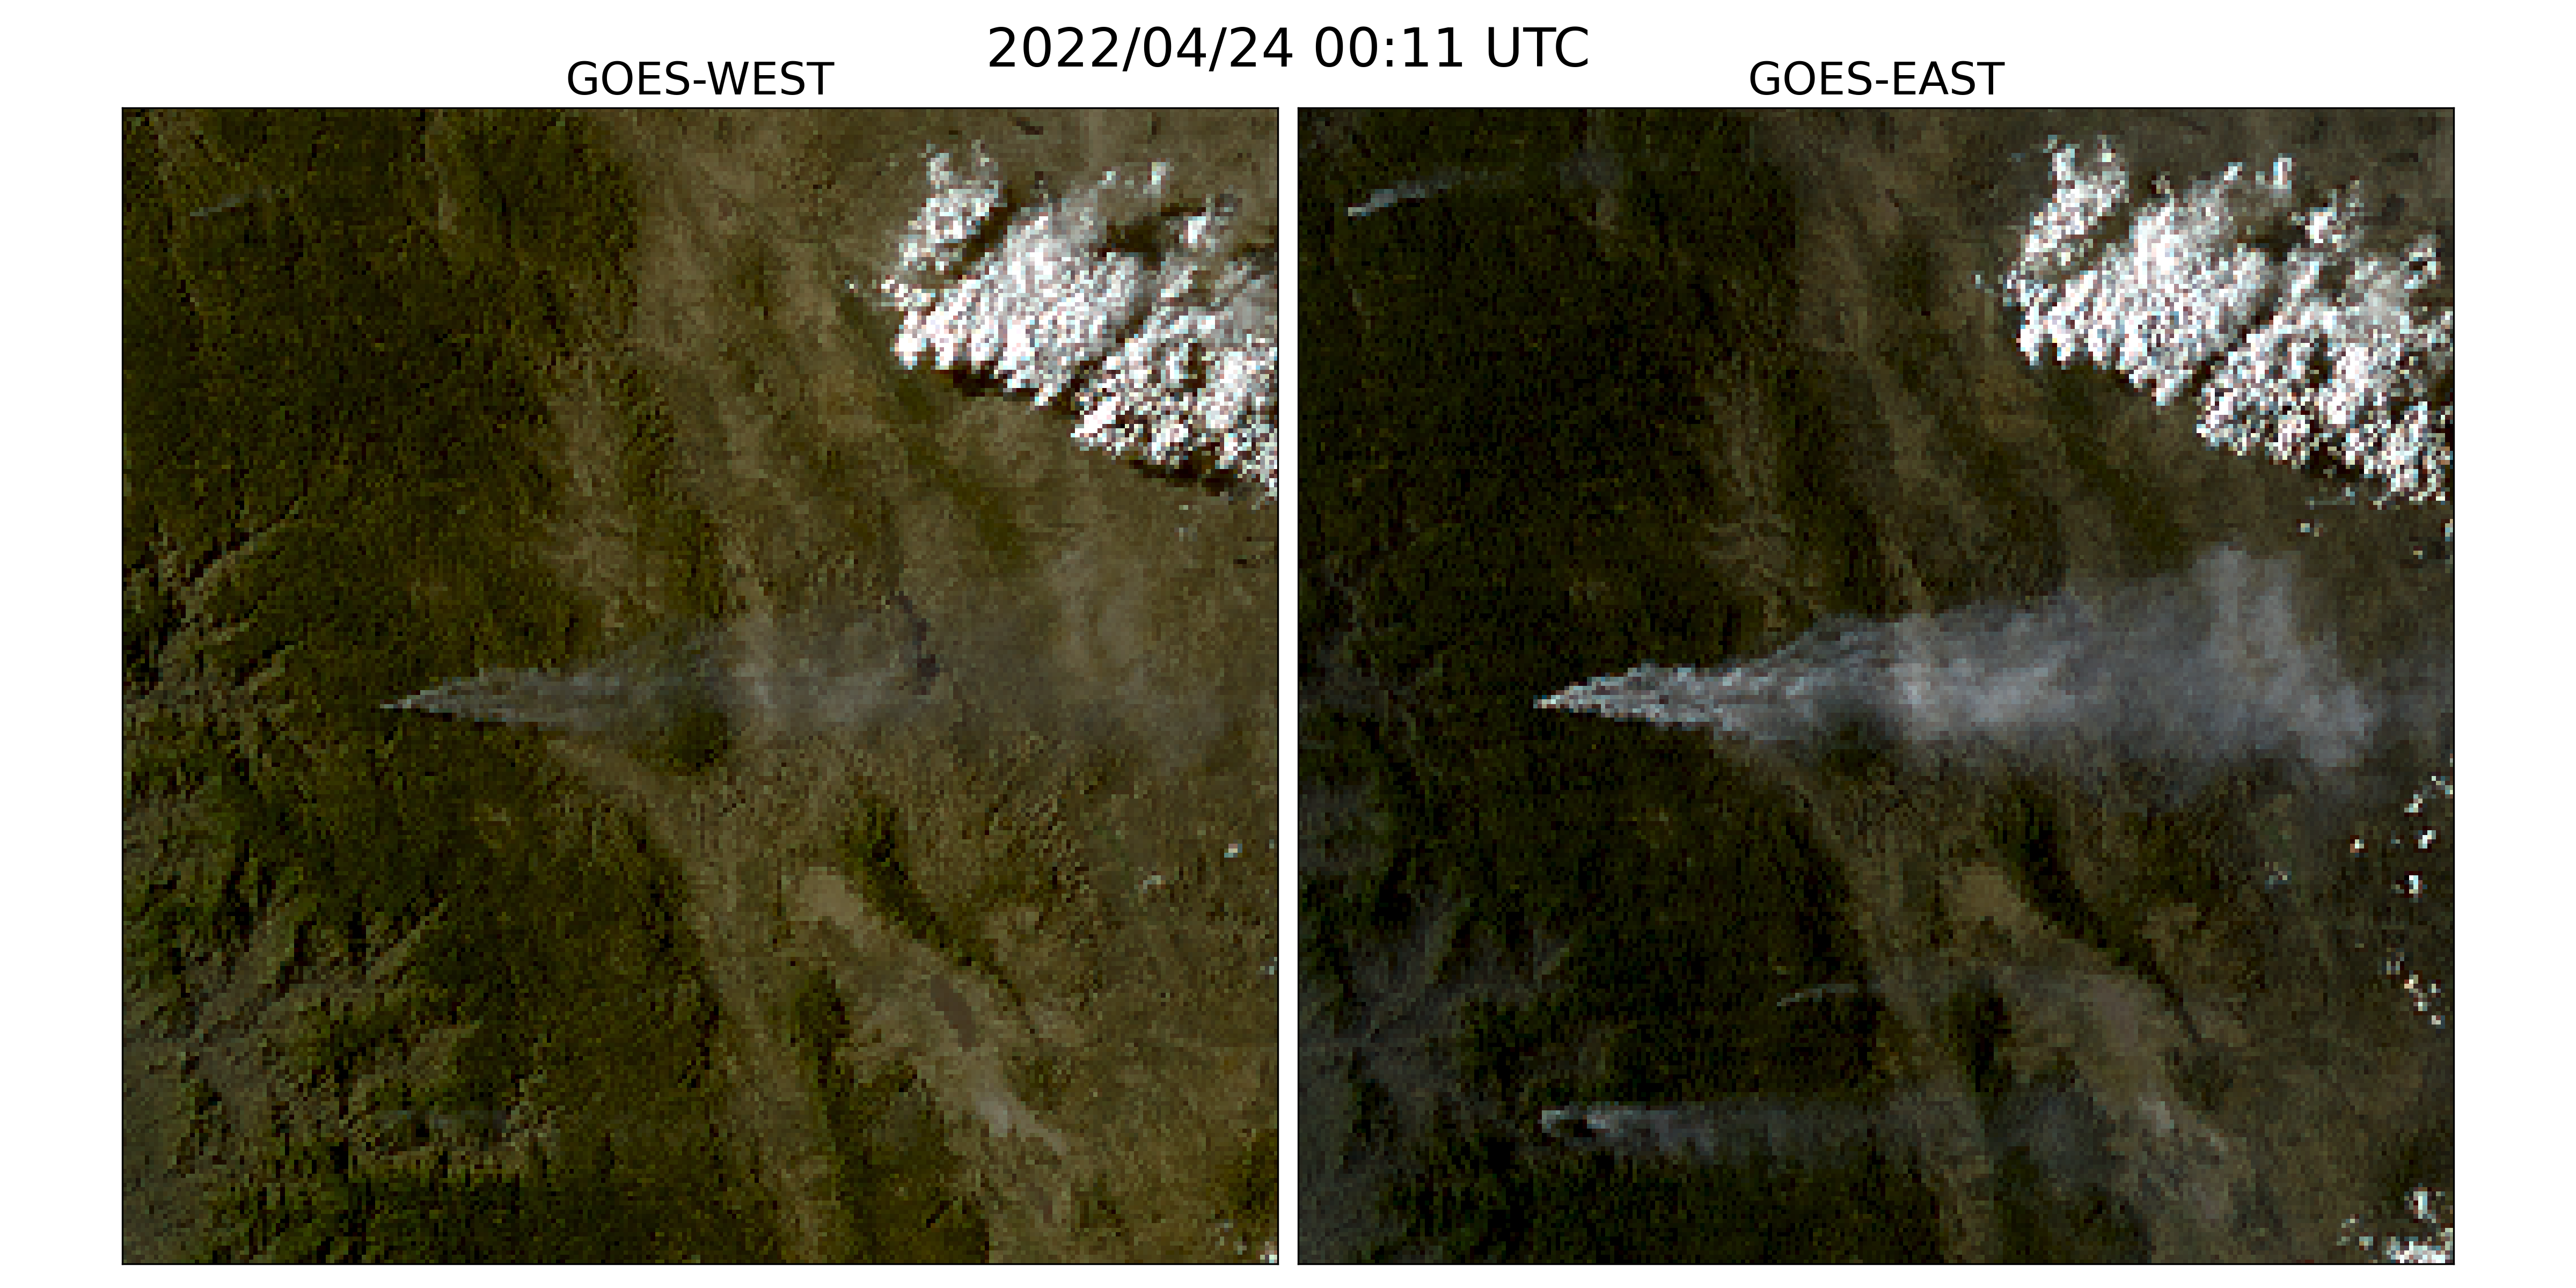
\includegraphics[width=8.5cm]{figures/G16_v_G17_2.png}
    \caption{True color GOES-West (left) and GOES-East (right) imagery from April \(24^{th}\), 2022 in Durango, Mexico. The images were taken \(\sim1.5\) hours before sunset (01:43 UTC) for this geolocation and time of year.}\label{16_vs_17}
\end{figure}

Smoke identification therefore amounts to extracting a signal of \(d > \lambda\) photons from the \(\lambda \gg d\) background. Positioning a detector along line of sight to the scatterer will result in a higher signal from smoke particles (figure \ref{mei}). Filtering the imaged wavelength can enhance this signal; photons collected in the blue spectrum will have a naturally lower background along the line of sight to the illumination source do their high level of Rayleigh scattering as. Therefore, as demonstrated in figure \ref{bands}, this configuration results in the highest signal to noise imaging for smoke particles.

\begin{figure}
    \centering
    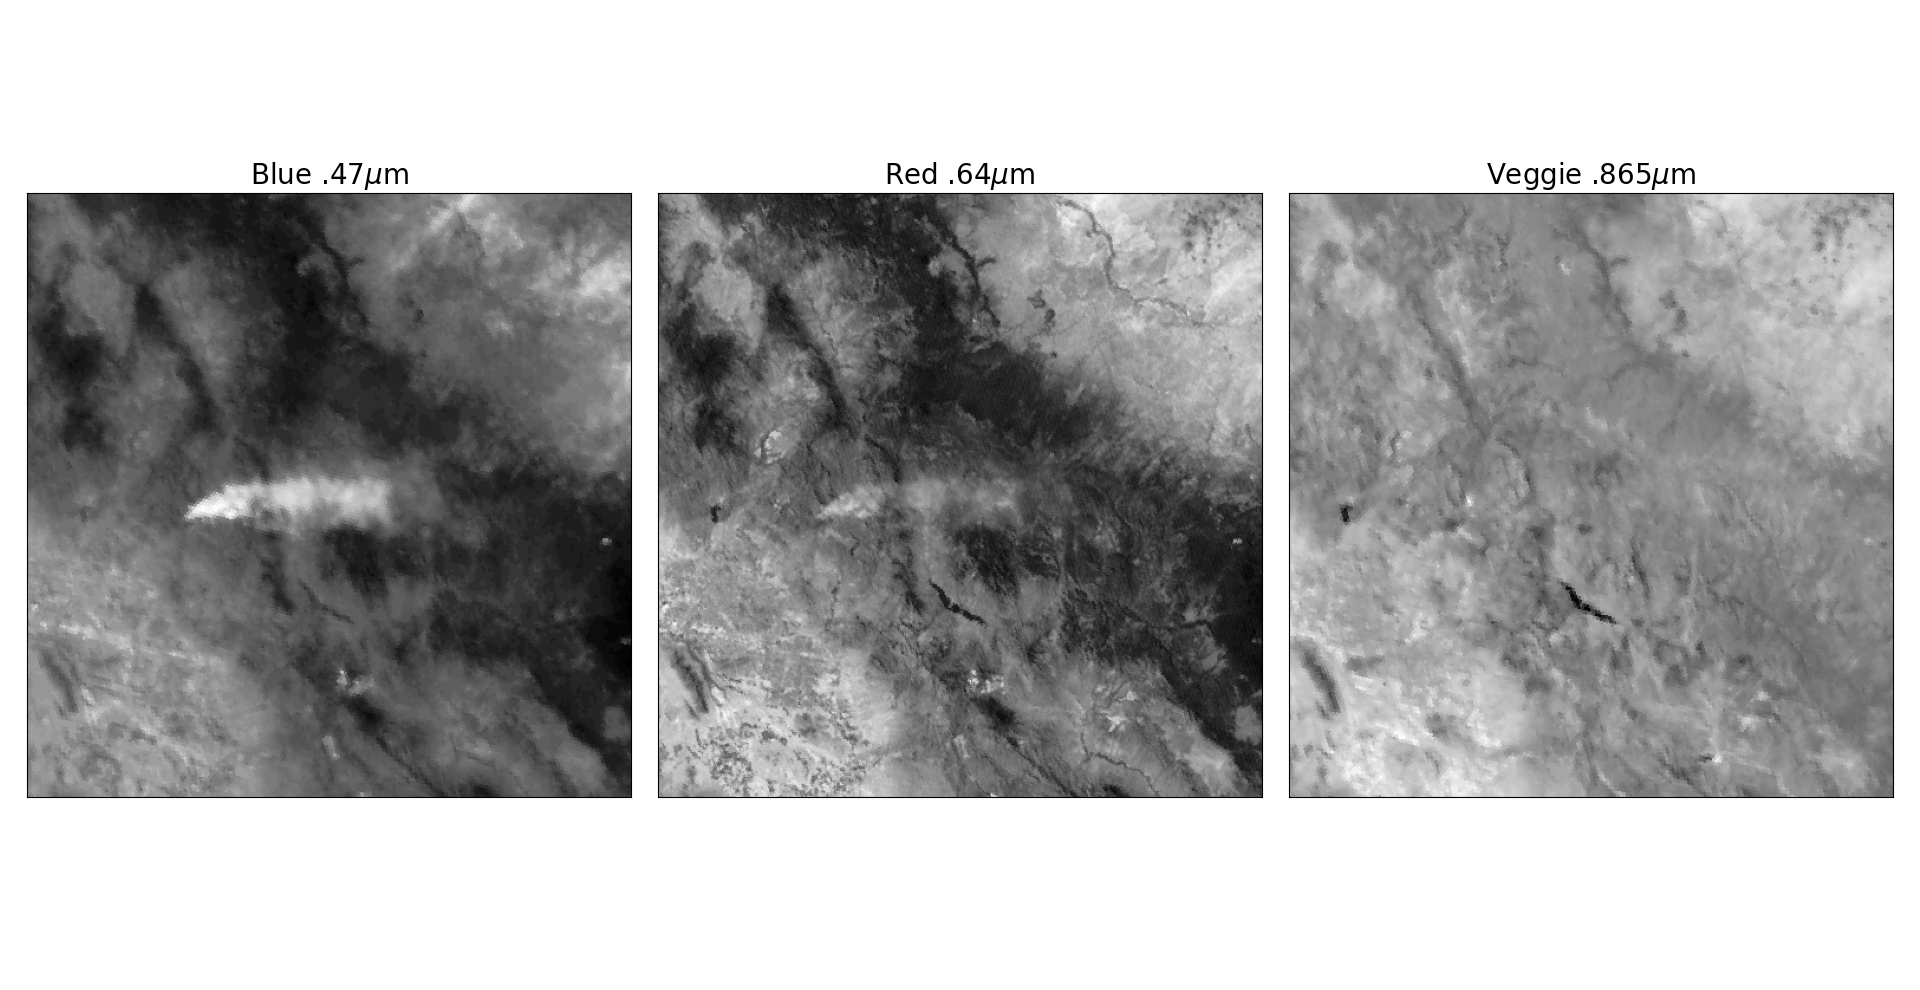
\includegraphics[width=8cm]{figures/GOES16_bands.png}
    \caption{Three bands of GOES-East data are the raw input to generate a true color image. These plots show variations in the signal-to-noise ratio for smoke detection in relation to the \(\lambda\) of light being measured.}\label{bands}
\end{figure}

Based solely on these criteria, the optimal strategy would be to pull data from GOES-West right after sunrise and from GOES-East right before sunset. Another factor to consider is that the time when the sun is in optimal alignment with the satellite for smoke detection coincides with when solar zenith angle is close to \(90^{\circ}\). Larger angles between the satellite and sun result in an increase in noise due to increased atmospheric interactions \cite{zen_angle}. To reduce the noise from large solar zenith angles, if given multiple frames to choose from, we choose the image with the largest solar zenith angle that is \(<88^{\circ}\).

The resulting image selection process takes into account atmospheric properties and light scattering physics to generate an estimate of which singular satellite image within the analyst time-window could give the highest smoke signal-to-noise ratio. The resulting Mie-derived dataset, \(\mathcal{X}_M = \{X_M, Y\}\), was then used to train a model, \(f_{\circ}\), that would generate \(N\) pseudo-labels, \(y^*\), for every sample, where \(N\) is determined by how many images, taken at a 10 minute interval, fit within the analyst time-window for that sample. Chosen from the \(N\) images, \(x_p\) is the image with the highest alignment between the \(f_{\circ}\) prediction of smoke, \(y^*\), in the image and the HMS analysts' annotation \(y\).

\subsubsection{Thermometer Encoding Smoke Densities}

One of the challenges introduced with using human generated qualitative smoke densities was that, as seen in figure \ref{densities}(c)-\ref{densities}(e) , there are variations in what is labeled as heavy or light density smoke. More generally, reproducing qualitative metrics with quantitative algorithms is a challenging problem, but we apply mathematical approaches that mitigate some of the underlying complications of our specific problem. Despite the smoke densities introduce qualitative complexities, we decided that the density approximations were important to use in our dataset because of the differences in signatures the densities produce. Within the satellite imagery, the appearance of a light density smoke plume will look significantly different than a heavy density smoke plume as seen in figure \ref{densities}. Additionally, a light density smoke plume is expected to be more challenging to detect since it is easier for it to be misclassified as not smoke. During the training process, the separate density categories allows us to deferentially weight the penalization given to the model for incorrect classifications based on category. For example, the model can be given a small penalization for misclassifying light smoke as not smoke while given a higher penalization for misclassifying heavy smoke as not smoke. 

In addition to the densities being ordered and categorical, the differences between the density categories are not evenly distributed by a given metric, such as PM\textsubscript{2.5} density. The intervals between densities being unknown along with the hierarchical nature of the density labels makes the labels ordinal instead of just categorical. This data property allows us to use thermometer encoding \cite{therm_enc}, which leverages the idea that heavy density smoke includes both medium and light density smoke, that heavy density smoke is closer to medium than it is to light, and automatically weights the loss functions and incorporates the ranked ordering of the densities. As seen in Table \ref{therm}, one-hot encoding, commonly used for categorical data, doesn't take ordinal properties of the data into consideration.

\begin{table}[h] 
    \caption{A comparison of one-hot encoding used for categorical data to thermometer encoding for ordinal data.}\label{therm}
    \centering
    \begin{tabular}{ccccrrcrc}
        \toprule
        category & one-hot & thermometer \\
        \midrule
        No Smoke & \texttt{[0 0 0]} & \texttt{[0 0 0]} \\
        Light  & \texttt{[0 0 1]} & \texttt{[0 0 1]} \\
        Medium & \texttt{[0 1 0]} & \texttt{[0 1 1]} \\
        Heavy  & \texttt{[1 0 0]} & \texttt{[1 1 1]} \\
        \bottomrule
    \end{tabular}
\end{table}

\subsubsection{Pseudo-label Dataset} 

We implement a deep learning architecture that uses the encoder from EfficientNetV2 \cite{efficientnetv2} and a semantic segmentation classifier from the DeepLabV3 model \cite{deeplab}. Transfer learning has shown to reduce the time and resources needed to train a model by leveraging information from pre-trained models \cite{transfer}, \cite{transfer2}. We initialize the values of our model weights using the pre-trained values originally trained on the ImageNet dataset \cite{imgnet}, containing 1.2 million images and 1000 categories. Our model was developed using the Segmentation Models PyTorch package \cite{semantic} that was written as a high level API for implementing models for semantic segmentation problems. We input 256x256x3 snapshots of 1km resolution true color GOES imagery that contains smoke and output a 256x256x3 classification map that predicts if a pixel contains smoke and if so, what the density of that smoke is. As mentioned earlier, we apply the thermometer encoding shown in table \ref{therm} to encode the smoke densities and apply binary cross entropy as the loss function per density of smoke. 

The dataset, \(\mathcal{X}_M\), contains 207,106 samples as shown in the dataset split in table \ref{split}. 

\begin{table}[h] 
    \caption{Dataset split for \(\mathcal{X}_M\) and \(\mathcal{X}_p\), samples for 2024 go up to November 1st. We use an entire year of data for both validation and testing sets to capture year-long wildfire trends.}\label{split}
    \centering
    \begin{tabular}{ccccrrcrc}
        \toprule
        dataset & \(\mathcal{X}_M\) & \(\mathcal{X}_p\) &years\\
        \midrule
        training & 165,609 & 144,225 &2018-2021, 2024\\
        validation & 20,056 & 19,223 &2023 \\
        testing & 21,541 & 20,224 & 2022 \\
        \bottomrule
    \end{tabular}
\end{table}

To determine which image out of the relevant imagery for the given time window best represents the analyst annotation, we implement a greedy algorithm by running \(f_{\circ}\) on each \(x\) to generate a pseudo-label, \(y^*\). The output of \(f_{\circ}\), \(y^*\) give predictions on if smoke is in the image, and if there is smoke, where the smoke is in that image and the density of that smoke. \(y^*\) serve as pseudo-labels for each density of smoke and are compared to the analyst annotations, \(y\). To compare \(y^*\) and \(y\), we calculate the IoU using the total set of pixels for \(y^*\) at that density of smoke and the entire set of pixels for \(y\) for a particular smoke density in each image as shown in equation \ref{overall_iou}. The image with the highest IoU score is chosen as the image, \(x_p\), that best represents the analyst smoke annotation, \(y\). Often used for pseudo-labeling, a confidence threshold value is defined to determine if a pseudo-label should to be included in a dataset \cite{conf_thresh}. We chose a confidence threshold that would include the sample, \(x_p\), in \(\mathcal{X}_{p}\) if the maximum overall IoU (equation \ref{overall_iou}) between \(y^*\) and \(y\) over all densities was over 0.01. 

\begin{equation} \label{overall_iou}
    IoU_{\text{overall}} = \frac{\sum\limits_{i=\text{light}}^{\text{heavy}}|y_{i}\cap y^*_{i}|}{\sum\limits_{i=\text{light}}^{\text{heavy}}|y_{i}|\cup|y^*_{i}|}
\end{equation}

We use \(\mathcal{X}_{p}\) to train an additional child model, \(f_c\) in order to assess if training with \(\mathcal{X}_{p}\) can produce a more robust semantic segmentation model compared to training on \(\mathcal{X}_M\). We use the same dataset split method and model setup but change \(\mathcal{X}_M\) to \(\mathcal{X}_{p}\) to train \(f_c\).

\subsection{Benchmark Models}

While this dataset is anticipated to be primarily useful for solving various wildfire smoke applications, this dataset could be a uniquely insightful test case for remote sensing semantic segmentation. Many deep learning satellite image datasets are focused on objects with sharp contrasts such as crops \cite{crops}, human infrastructure \cite{polyworld}, or even clouds over oceans \cite{cyclone, cloud_texture}, but smoke has indistinct boundaries that often fade both spatially and temporally.

We benchmark the SmokeViz dataset, \(\mathcal{X}_{p}\) by varying the semantic segmentation classification heads. We train Linknet \cite{linknet}, PSPNet \cite{pspnet} and MANet \cite{manet} using the same encoder used for \(f_c\) and \(f_{\circ}\), EfficientNetV2. Each model is trained over 100 epochs using a batch size of 32 and the Adam optimizer on 8 Nvidia P100 GPUs allocating 100GB of memory over 12 hours of allotted training time. We choose these architectures because of their abilities to capture multi-scale objects such the varying spatial extents of smoke plumes.



